\subsection{Straßenverkehrsschilder}
In diesem Abschnitt soll eine kurze Definition von Straßenverkehrsschildern sowie eine Vorstellung der in Deutschland geltenen Rechtslage (Rechtslage im Bezug auf was? evtl. kurz erläutern) gegeben werden. Außerdem wird ein Überblick, über den verwendeten (das ist einer deiner Lieblingswörter :D versuche ab und an Synonyme zu nutzen;) \ac{GTSRB} Datensatz gegeben.

\subsubsection{Straßenverkehrsschilder in Deutschland}
Straßenverkehrsschilder dienen dazu, den Straßenverkehr zu regeln. Hierbei stellen sie den Verkehrsteilnehmern Warnungen, Informationen und Einzelheiten über Einschränkungen zur Verfügung. (Das klingt bis hier hin so schön freiwillig :D) Sie fallen dabei unter die Straßenausstattung und werden behördlich angeordnet. \todo{Beleg} Alle gültigen Straßenverkehrsschilder in Deutschland werden in der \ac{StVO} gelistet. Diese wird fortlaufend den aktuellen Gegebenheiten angepasst und durch Novellen aktualisiert. Grundsätzlich basieren die Straßenverkehrsschilder dabei auf dem am 8. November 1968 in Wien beschlossenen \textit{Übereinkommen über den Straßenverkehr} (engl. Originaltitel "Convention on Road Traffic").\footcite[Vgl.][o.S.]{unConventionRoadTraffic1977} 
 Dieses wurde bis heute von 36 Nationen unterzeichnet und von 84 Nationen ratifiziert.\footcite[Vgl.][1-14]{unUnitedNationsTreaty2020}

In der \ac{StVO} sind drei Gruppen von Verkehrszeichen definiert:
\begin{itemize}
    \item Gefahrenzeichen (§ 40 \ac{StVO})
    \item Vorschriftzeichen (§ 41 \ac{StVO})
    \item Richtzeichen (§ 42 \ac{StVO})
\end{itemize}

(Die Platzierung der Tabelle macht hier noch nicht so viel Sinn) Neben diesen Verkehrszeichen gibt es noch Zusatzzeichen, welche zusammen mit Zeichen aus den genannten Gruppen verwendet werden. Diese sind in § 39 Abs. 7 \ac{StVO} aufgelistet.


\subsubsection{German Traffic Sign Recognition Benchmark}
Für den praktischen Teil dieser Arbeit, wird ein Datensatz von Straßenverkehrsschildern benötigt, mit denen das \ac{CNN} initial trainiert und bewertet werden kann. Es gibt eine Vielzahl von Datensätzen die hierfür potentiell in Frage kommen/ geeignet wären. Das \textit{\ac{MASTIF}} Projekt stellt drei verschiedene Datensätze aus den Jahren 2009, 2010 und 2011 zur Verfügung. Der umfangreichste ist hierbei der Datensatz aus 2009 mit 6000 Bildern.\footcite[Vgl.][S. 66-73]{vsegvic2010computer} Shakhuro und Konushin stellen einen Datensatz mit 104.358 verschiedenen russischen Schildern aus dem Jahre 2016 zur Verfügung. (Ist diese Information für den Leser nützlich? Wenn nicht, streiche den Satz)\footcite[Vgl.][S. 294-300]{rtsd} Der bisher umfangreichste Datensatz ist das \textit{Mapillary Traffic Sign Dataset} aus dem Jahre 2020. Es enthält 100.000 Bilder mit insgesamt 325.172 erkannten Schildern. Von diesen Schildern Fallen 82.724 Schilder in die im Datensatz gekennzeichneten Schilderklassen. Die Bilder stammen dabei aus der ganzen Welt, eine grobe Verteilung liegt bei 20\% Nordamerika, 20\% Europa, 20\% Asien, 15\% Südamerika, 15\% Ozeanien und 10\% Afrika.\footcite[Vgl.][S. 1-17]{ertlerMapillaryTrafficSign2020}

\begin{table}[t]
    
    \caption{Übersicht der fünf besten (das Wort "beste" ist hier nicht weiter definiert- würde ich evtl durch "genausten" ersetzen)Einreichungen GTSRB Klassifizierung\label{table:TopGTRSBPaper}} 
    \resizebox{\textwidth}{!}{%
    \begin{tabular}{@{}llc@{}}
    \toprule
    \textbf{Team}                                        & \textbf{Methode}                                           & \begin{tabular}[c]{@{}c@{}}\textbf{Prozentzahl} \\ \textbf{(Genauigkeit)}\end{tabular} \\ \midrule
    Arcos-García, Álvarez-García, Soria-Morillo & CNN mit 3 Spatial Transformers                    & 99.71                                                                \\
    Ciresan, Meier, Masci, Schmidhuber         & Zusammenschluss mehrerer CNNs                     & 99.46                                                                \\
    Gecer, Azzopardi, Petkov                  & Farbenbasierter COSFIRE-Filterzur Objekterkennung & 98.97                                                                \\
    Stallkamp, Schlipsing, Salmen, Igel & Durchschnittliches menschliches Abschneiden & 98.84 \\
    Sermanet, LeCun                            & Mehrstufige CNNs                                  & 98.31                                                                \\ \bottomrule
    \end{tabular}%
    }
    
    \hfill \break
    Quelle: In Anlehnung an Institut für Neuroinformatik Ruhr-Universität Bochum, Resultate GTSRB, 2019, o.S.
\end{table} 
Letztendlich wurde sich für den Datensatz \ac{GTSRB} entschieden. Dieser umfasst 51.840 Bilder von 1700 verschiedenen deutschen Straßenverkehrsschilder, welche in 43 Klassen unterteilt wurden. Grund für die Auswahl war primär, dass dieser Datensatz die größte Anzahl von deutschen Straßenverkehrsschilder liefert/ bereitstellt, auf denen  der Schwerpunkt dieser Arbeit liegt (Irgendwas stört mich an dem Satz, habe aber spontan auch keinen besseren Vorschlag). Der Datensatz wurde im Jahre 2010 erstellt und die Maße der Bilder variieren zwischen 15x15 und 222x193 Pixeln. In Abbildung \ref{fig:overviewClassesGTSRB} wird die Anzahl der Bildern pro Klasse im Trainingsdatensatz des \ac{GTSRB} dargestellt. Die 43 Klassen des Datensatzes fallen alle unter die drei Gruppen der Verkehrszeichen nach § 39 Abs. 2 Satz 2 \ac{StVO}. Dabei fallen 27 Klassen unter Vorschriftzeichen, 14 Klassen unter Gefahrenzeichen und 2 Klassen unter Richtzeichen (Das würde ich noch ins Glossar packen). 
Für den \ac{GTSRB} liegen eine Vielzahl von Forschungsarbeiten vor.\footcite[Vgl.][S. 158 - 165]{arcos-garciaDeepNeuralNetwork2018}\footcite[Vgl.][165-174]{gecerColorblobbasedCOSFIREFilters2017}\footcite[Vgl.][S. 333-33]{ciresanMulticolumnDeepNeural2012}\footcite[Vgl.][S. 323-332]{Stallkamp2012}\footcite[Vgl.][S. 2809-2813]{sermanetTrafficSignRecognition2011} Die fünf Einreichungen mit der höchsten \textit{Accuracy} (Genauigkeit) auf dem Testdatensatz sind in Tabelle \ref{table:TopGTRSBPaper} aufgelistet. Es ist zu erkennen, dass bereits eine sehr hohe Accuracy erreicht wird (99.71\%). 


\begin{figure}[t]
    \centering
    \caption[]{Anzahl Bilder pro Klasse im GTSRB Trainingsdatensatz}
	\label{fig:overviewClassesGTSRB}
    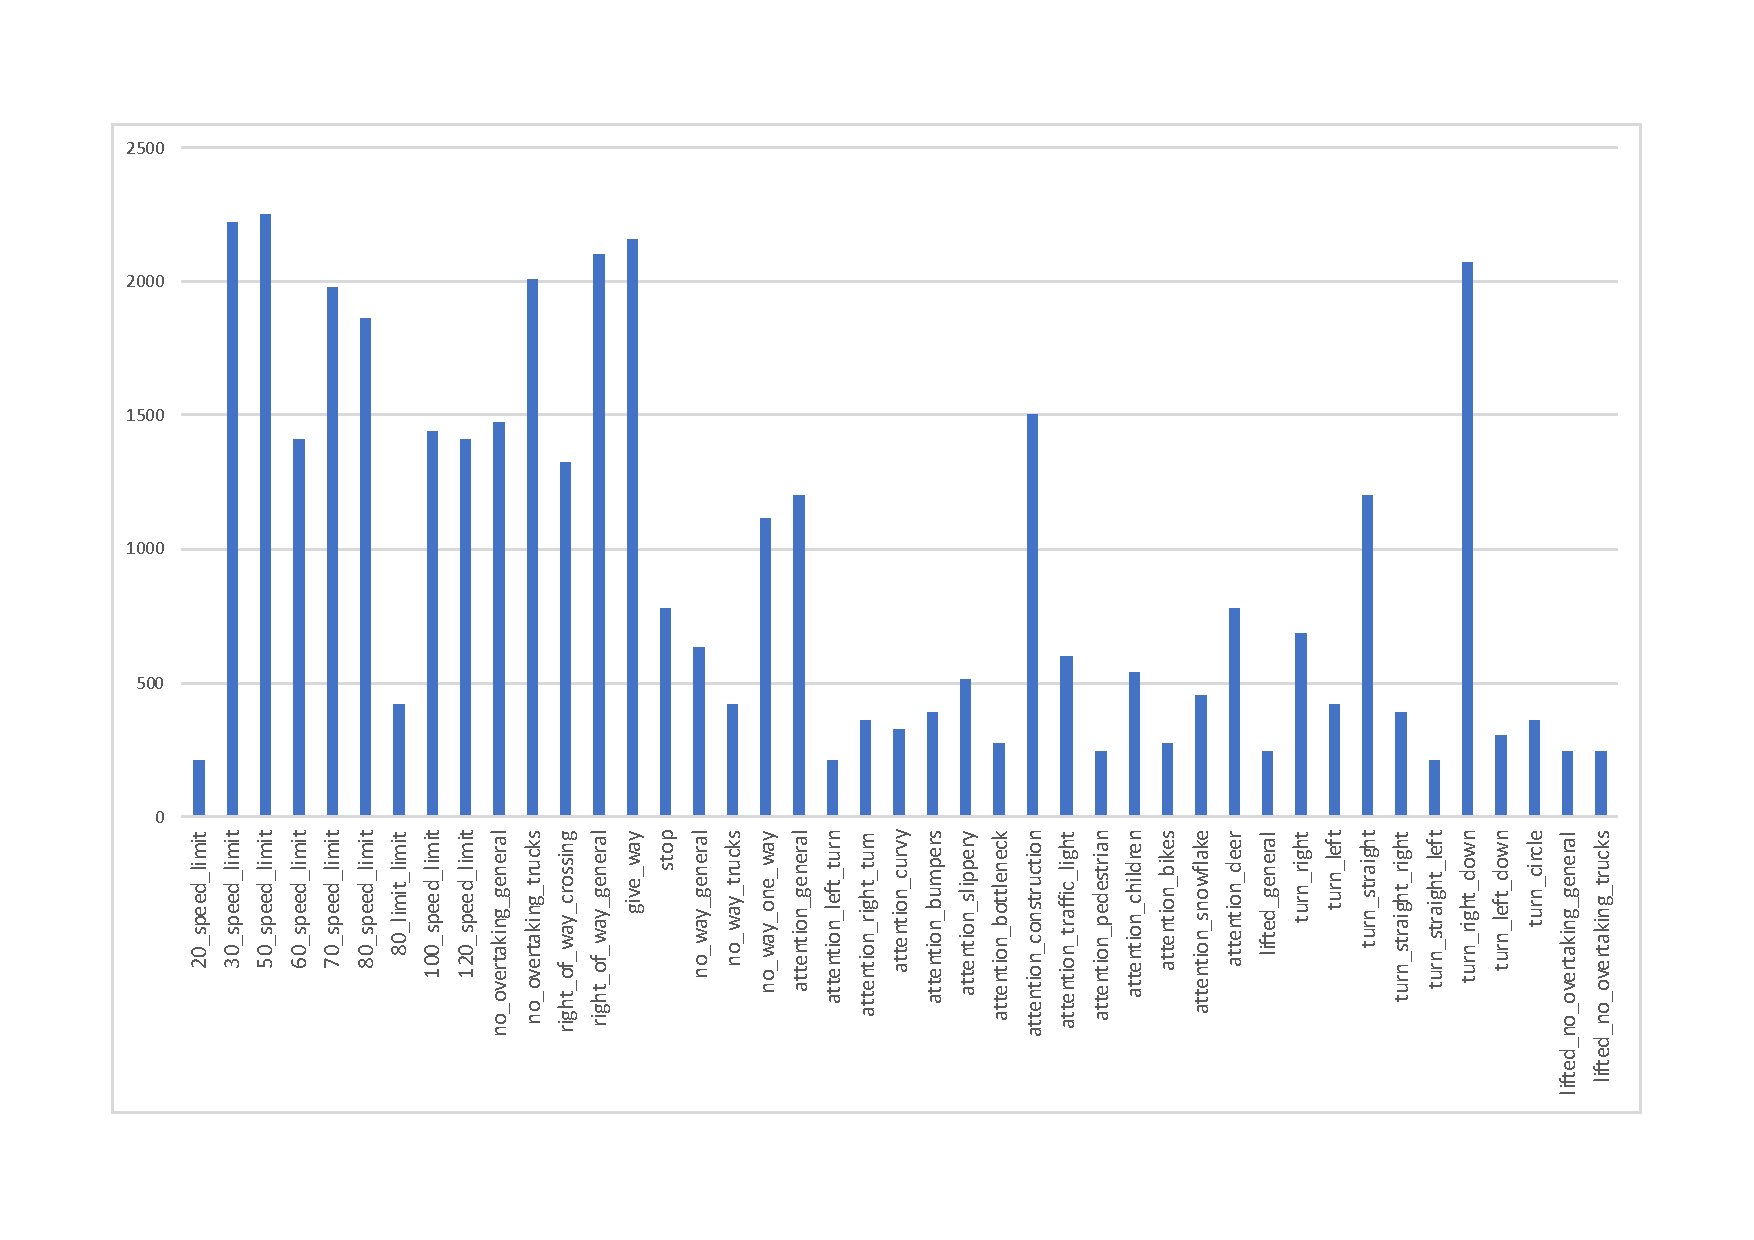
\includegraphics[width=1\textwidth]{image_per_class.pdf}
    Quelle: Eigene Darstellung, 2020
\end{figure}


